\chapter{Social Media as Recruiting Leverage}

This chapter follows a short School of Hard Knocks entrepreneurship interview segment curated by LazyingArt LLC for Video2Book. The transcript asks one narrow question: how important has a social-media following been as leverage? The answer is not built as a theory of media. It is built as a small business observation: a moderate audience created enough company visibility that some new hires discovered the firm through Grant's TikTok presence.

\section{The Opening Question}

The exchange begins with a clean entrepreneurial question. We are not first asking whether social media is popular, or whether followers create status. We are asking whether the following has been useful as leverage.

\subsection{Question \& Answer}

\paragraph{Question.}
How important has leveraging the social-media following been?

\paragraph{Answer.}
The answer given in the interview is immediate: it has been huge. But the useful part of the answer is the way the speaker supports it. He does not claim to have a massive celebrity-scale audience. He gives the scale, then moves quickly to a hiring example.

The logical structure is therefore simple:

\begin{equation}
\text{following} \quad \longrightarrow \quad \text{visibility} \quad \longrightarrow \quad \text{business consequence}.
\end{equation}

For this excerpt, the business consequence is recruiting. The following makes the company visible to people who might otherwise never have encountered it.

\section{A Modest Audience With Business Consequences}

The speaker gives two follower counts. TikTok is the larger platform in the example, and Instagram is smaller:

\begin{align}
F_T &\approx 145{,}000,\\
F_I &\approx 25{,}000.
\end{align}

Here \(F_T\) denotes the TikTok following and \(F_I\) denotes the Instagram following. The combined stated audience is therefore approximately

\begin{equation}
F_T + F_I \approx 145{,}000 + 25{,}000 = 170{,}000.
\end{equation}

That number is large enough to matter, but the speaker explicitly frames it as not massive. This is the first important business point. The claim is not that only enormous media figures can benefit from attention. The claim is that a focused audience can create practical surface area for a company.

\begin{remark}
The transcript supports the follower counts and the speaker's qualification that the following is not massive. It does not support a conversion-rate model from total followers to total hires. The arithmetic here should be read as scale-setting, not as a measured funnel.
\end{remark}

\section{The Company Meeting Test}

The interview then pivots from audience size to evidence. The speaker describes a company-wide meeting held the previous Monday. Six or seven people were starting, and a director asked them to explain how they found the company and how they got the job.

Let

\begin{equation}
N \in \{6,7\}
\end{equation}

be the number of new starters in that meeting. The small size matters. We are not looking at a large statistical sample. We are looking at a concrete internal moment where the company heard where new people came from.

The structure of the evidence is anecdotal but still operationally useful. The company asks new hires how they arrived. Some of the answers point back to social media. The transcript names locations such as Portland, Tennessee, and Florida, which makes the point more specific: the media presence was not merely local reputation. It reached people distributed across different places.

\section{Recruiting Attribution}

The key quantitative claim is that roughly 30 to 40 percent of those new starters said they had been following Grant:

\begin{equation}
p \approx 30\%\text{--}40\%.
\end{equation}

Here \(p\) is the share of the new-starter group whose awareness was attributed, in the meeting, to following Grant. If we apply that range to the stated cohort size, the implied count is small but concrete.

\subsection{A Cautious Arithmetic Example}

The transcript does not state an exact count. It gives a cohort size and a percentage range. The cautious reconstruction is:

\begin{align}
H &\approx pN,\\
H &\approx (0.30\text{--}0.40)(6\text{--}7),\\
H &\approx 1.8\text{--}2.8.
\end{align}

So in ordinary business language, the statement points to about two or three new people in that small starting group.

This is not a law of hiring. It is not a proof that every 170,000 followers yields a fixed number of hires. It is a concrete example of leverage: attention that already existed outside the firm became a path by which talent found the firm.

\section{The Mechanism}

The final movement in the transcript is the mechanism. Someone follows Grant on TikTok for six months. Then the person sees a job. Then, suddenly, the company has a talented person working inside it who might never have seen the company without social media.

We can write that mechanism as a narrow sequence rather than a broad marketing slogan.

\begin{figure}
\centering
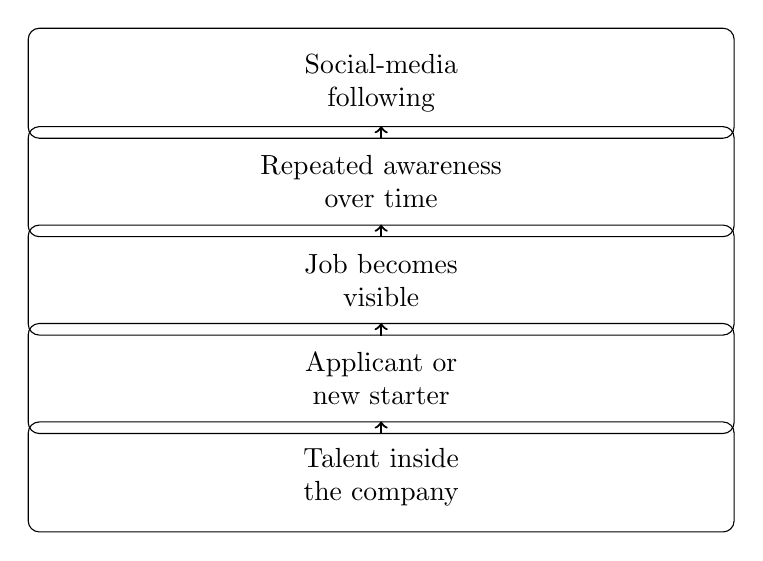
\begin{tikzpicture}[
  box/.style={draw, rounded corners, align=center, text width=0.72\linewidth, minimum height=0.55in},
  arrow/.style={->, thick}
]
\node[box] (a) at (0,0) {Social-media\\following};
\node[box] (b) at (0,-1.25) {Repeated awareness\\over time};
\node[box] (c) at (0,-2.50) {Job becomes\\visible};
\node[box] (d) at (0,-3.75) {Applicant or\\new starter};
\node[box] (e) at (0,-5.00) {Talent inside\\the company};

\draw[arrow] (a) -- (b);
\draw[arrow] (b) -- (c);
\draw[arrow] (c) -- (d);
\draw[arrow] (d) -- (e);
\end{tikzpicture}
\caption{Transcript-derived mechanism: social attention becomes recruiting visibility.}
\end{figure}

The important phrase is not simply ``followers.'' Followers are a stock. The business effect comes from a flow: attention turns into awareness, awareness turns into discovery, and discovery can turn into a hire.

We can summarize that distinction as

\begin{equation}
\text{media leverage}
=
\text{audience stock}
\times
\text{credible repeated exposure}
\times
\text{available opportunity}.
\end{equation}

This is a reconstruction of the mechanism, not a formula measured in the interview. Its purpose is to keep the reasoning straight. The audience alone does not hire anyone. The job posting alone may not reach the right person. The useful leverage appears when the audience has been warmed by repeated exposure and then sees an opportunity at the right time.

\section{Summary}

The excerpt gives a compact lesson about entrepreneurial leverage through media. Grant names a following of about \(145{,}000\) on TikTok and \(25{,}000\) on Instagram, while insisting that this is not an enormous audience. The practical evidence is a company meeting with six or seven new starters, where roughly 30 to 40 percent reportedly traced their awareness to following him.

The careful conclusion is modest but important. Social media is not presented here as abstract fame. It is presented as a recruiting surface. A person can follow for months, see an opening, and become part of the company. For an entrepreneur, that is leverage: prior attention converted into opportunity flow.